% Options for packages loaded elsewhere
\PassOptionsToPackage{unicode}{hyperref}
\PassOptionsToPackage{hyphens}{url}
%
\documentclass[
  ignorenonframetext,
]{beamer}
\usepackage{pgfpages}
\setbeamertemplate{caption}[numbered]
\setbeamertemplate{caption label separator}{: }
\setbeamercolor{caption name}{fg=normal text.fg}
\beamertemplatenavigationsymbolsempty
% Prevent slide breaks in the middle of a paragraph
\widowpenalties 1 10000
\raggedbottom
\setbeamertemplate{part page}{
  \centering
  \begin{beamercolorbox}[sep=16pt,center]{part title}
    \usebeamerfont{part title}\insertpart\par
  \end{beamercolorbox}
}
\setbeamertemplate{section page}{
  \centering
  \begin{beamercolorbox}[sep=12pt,center]{part title}
    \usebeamerfont{section title}\insertsection\par
  \end{beamercolorbox}
}
\setbeamertemplate{subsection page}{
  \centering
  \begin{beamercolorbox}[sep=8pt,center]{part title}
    \usebeamerfont{subsection title}\insertsubsection\par
  \end{beamercolorbox}
}
\AtBeginPart{
  \frame{\partpage}
}
\AtBeginSection{
  \ifbibliography
  \else
    \frame{\sectionpage}
  \fi
}
\AtBeginSubsection{
  \frame{\subsectionpage}
}
\usepackage{amsmath,amssymb}
\usepackage{lmodern}
\usepackage{ifxetex,ifluatex}
\ifnum 0\ifxetex 1\fi\ifluatex 1\fi=0 % if pdftex
  \usepackage[T1]{fontenc}
  \usepackage[utf8]{inputenc}
  \usepackage{textcomp} % provide euro and other symbols
\else % if luatex or xetex
  \usepackage{unicode-math}
  \defaultfontfeatures{Scale=MatchLowercase}
  \defaultfontfeatures[\rmfamily]{Ligatures=TeX,Scale=1}
  \setmainfont[BoldFont = SF Pro Rounded Semibold]{SF Pro Rounded}
  \setmathfont[]{STIX Two Math}
\fi
\usefonttheme{serif} % use mainfont rather than sansfont for slide text
% Use upquote if available, for straight quotes in verbatim environments
\IfFileExists{upquote.sty}{\usepackage{upquote}}{}
\IfFileExists{microtype.sty}{% use microtype if available
  \usepackage[]{microtype}
  \UseMicrotypeSet[protrusion]{basicmath} % disable protrusion for tt fonts
}{}
\makeatletter
\@ifundefined{KOMAClassName}{% if non-KOMA class
  \IfFileExists{parskip.sty}{%
    \usepackage{parskip}
  }{% else
    \setlength{\parindent}{0pt}
    \setlength{\parskip}{6pt plus 2pt minus 1pt}}
}{% if KOMA class
  \KOMAoptions{parskip=half}}
\makeatother
\usepackage{xcolor}
\IfFileExists{xurl.sty}{\usepackage{xurl}}{} % add URL line breaks if available
\IfFileExists{bookmark.sty}{\usepackage{bookmark}}{\usepackage{hyperref}}
\hypersetup{
  pdftitle={444 Lecture 8.5 - Real Life Stag Hunts},
  pdfauthor={Brian Weatherson},
  hidelinks,
  pdfcreator={LaTeX via pandoc}}
\urlstyle{same} % disable monospaced font for URLs
\newif\ifbibliography
\usepackage{graphicx}
\makeatletter
\def\maxwidth{\ifdim\Gin@nat@width>\linewidth\linewidth\else\Gin@nat@width\fi}
\def\maxheight{\ifdim\Gin@nat@height>\textheight\textheight\else\Gin@nat@height\fi}
\makeatother
% Scale images if necessary, so that they will not overflow the page
% margins by default, and it is still possible to overwrite the defaults
% using explicit options in \includegraphics[width, height, ...]{}
\setkeys{Gin}{width=\maxwidth,height=\maxheight,keepaspectratio}
% Set default figure placement to htbp
\makeatletter
\def\fps@figure{htbp}
\makeatother
\setlength{\emergencystretch}{3em} % prevent overfull lines
\providecommand{\tightlist}{%
  \setlength{\itemsep}{0pt}\setlength{\parskip}{0pt}}
\setcounter{secnumdepth}{-\maxdimen} % remove section numbering
\let\Tiny=\tiny

 \setbeamertemplate{navigation symbols}{} 

% \usetheme{Madrid}
 \usetheme[numbering=none, progressbar=foot]{metropolis}
 \usecolortheme{wolverine}
 \usepackage{color}
 \usepackage{MnSymbol}
% \usepackage{movie15}

\usepackage{amssymb}% http://ctan.org/pkg/amssymb
\usepackage{pifont}% http://ctan.org/pkg/pifont
\newcommand{\cmark}{\ding{51}}%
\newcommand{\xmark}{\ding{55}}%

\DeclareSymbolFont{symbolsC}{U}{txsyc}{m}{n}
\DeclareMathSymbol{\boxright}{\mathrel}{symbolsC}{128}
\DeclareMathAlphabet{\mathpzc}{OT1}{pzc}{m}{it}

\setlength{\parskip}{1ex plus 0.5ex minus 0.2ex}

\AtBeginSection[]
{
\begin{frame}
	\Huge{\color{darkblue} \insertsection}
\end{frame}
}

\renewenvironment*{quote}	
	{\list{}{\rightmargin   \leftmargin} \item } 	
	{\endlist }

\definecolor{darkgreen}{rgb}{0,0.7,0}
\definecolor{darkblue}{rgb}{0,0,0.8}

\usepackage[italic]{mathastext}
\usepackage{nicefrac}
\usepackage{istgame}

\setbeamertemplate{caption}{\raggedright\insertcaption}

%\def\toprule{}
%\def\bottomrule{}
%\def\midrule{}
\usepackage{etoolbox}
\AfterEndEnvironment{description}{\vspace{9pt}}
\AfterEndEnvironment{oltableau}{\vspace{9pt}}
\BeforeBeginEnvironment{oltableau}{\vspace{9pt}}
\AfterEndEnvironment{center}{\vspace{9pt}}
\BeforeBeginEnvironment{tabular}{\vspace{9pt}}
\AfterEndEnvironment{longtable}{\vspace{-6pt}}
\usepackage{booktabs}
\usepackage{longtable}
\usepackage{array}
\usepackage{multirow}
\usepackage{wrapfig}
\usepackage{float}
\usepackage{colortbl}
\usepackage{pdflscape}
\usepackage{tabu}
\usepackage{threeparttable} 
\usepackage{threeparttablex} 
\usepackage[normalem]{ulem} 
\usepackage{makecell}
\usepackage{xcolor}
\usepackage{ulem}

\setlength\heavyrulewidth{0ex}
\setlength\lightrulewidth{0.08ex}

\aboverulesep=0ex
\belowrulesep=0ex
\renewcommand{\arraystretch}{1.2}
\ifluatex
  \usepackage{selnolig}  % disable illegal ligatures
\fi

\title{444 Lecture 8.5 - Real Life Stag Hunts}
\author{Brian Weatherson}
\date{}

\begin{document}
\frame{\titlepage}

\begin{frame}{PD or Stag Hunt}
\protect\hypertarget{pd-or-stag-hunt}{}
So here's a depressingly common kind of situation.

\begin{itemize}
\tightlist
\item
  There is a social interaction where we'd all be better off if we all
  cooperated.
\item
  But for whatever reason, cooperation hasn't arisen. \pause
\item
  One question to ask, assuming people are rational, well-informed, etc,
  is whether this is more like PD or Stag Hunt.
\item
  In particular, if people did cooperate in this kind of situation,
  would cooperation be naturally sustainable, or would it require
  constant effort to sustain the cooperative equilibrium?
\end{itemize}
\end{frame}

\begin{frame}{Vague Question}
\protect\hypertarget{vague-question}{}
\begin{itemize}
\tightlist
\item
  There are, as always, borderline cases.
\item
  As Skyrms points out, there is a natural sense in which Iterated PD
  is, in the sense we're interested in, a Stag Hunt not a PD.
\item
  That's because mutual cooperation is, at least in the iterated game,
  an equilibrium.
\item
  But when there isn't a lot of iteration, and in particular when there
  isn't iteration between the same people over and over again, we're
  back in PD.
\end{itemize}
\end{frame}

\begin{frame}{Why This Matters}
\protect\hypertarget{why-this-matters}{}
\begin{enumerate}
\tightlist
\item
  We're theorists here and we like getting this kind of thing right!
\item
  The social reforms needed to develop, and sustain, a cooperative
  equilibrium in the two cases might be very different.
\end{enumerate}
\end{frame}

\begin{frame}{How Do We Tell}
\protect\hypertarget{how-do-we-tell}{}
\begin{itemize}
\tightlist
\item
  If we were in the cooperative state, would everyone have an incentive
  to stay in it, or would they still have a (small) incentive to defect.
\item
  In PD, everyone wants to defect even in the happy world where everyone
  else cooperates.
\item
  In Stag Hunt, once there is cooperation, cooperation is actually
  beneficial to the participants.
\end{itemize}
\end{frame}

\begin{frame}{Example One - Walking}
\protect\hypertarget{example-one---walking}{}
\begin{itemize}
\tightlist
\item
  So think about what it's like to walk through a crowded shared space:
  the corridors of a university, the common spaces of a shopping mall, a
  crowded sidewalk in a busy city.
\item
  There are more or less cooperative ways to walk. Roughly speaking, the
  straighter the line you walk in, and the closer your speed is to the
  median speed, the more cooperative you are. \pause
\item
  Some places are pretty cooperative. UM hallways are surprisingly so on
  the whole, and any major business city I've been in has been pretty
  cooperative during the morning and evening commute. \pause
\item
  But a lot of places are not - everyone is going in all directions, and
  it's a constant struggle to not get collided into many times. The
  touristy parts of big cities are like this all the time.
\end{itemize}
\end{frame}

\begin{frame}{PD or Stag Hunt}
\protect\hypertarget{pd-or-stag-hunt-1}{}
So question - if you're in one of the situations where things are going
well, is there an incentive to defect and try to cut through the crowds
even more quickly?
\end{frame}

\begin{frame}{My (very anecdotal) View}
\protect\hypertarget{my-very-anecdotal-view}{}
\begin{itemize}
\tightlist
\item
  This kind of feels like a Stag Hunt to me.
\item
  If you're somewhere where the pedestrian traffic is moving smoothly
  and quickly enough, there isn't much to gain by darting between people
  looking for a small edge. You just go with the traffic.
\item
  But if everyone is going at all angles and all speeds, then trying to
  be as cooperative as possible, sticking to a steady speed and a
  straight line, will be a disaster.
\item
  The best way to get where you're going (in a reasonable time with
  minimal risk) is to do what everyone else does.
\end{itemize}
\end{frame}

\begin{frame}{Example Two - Climate Change}
\protect\hypertarget{example-two---climate-change}{}
\begin{itemize}
\tightlist
\item
  Let's focus on climate change as an issue that affects the
  relationship between countries. (How individuals relate to each other
  vis a vis climate change is a trickier question.)
\item
  At this level it is often thought to be a PD (or what's sometimes
  called a free rider problem).
\item
  Everyone would prefer that everyone had lower emissions.
\item
  But everyone would prefer to not lower their own emissions.
\end{itemize}
\end{frame}

\begin{frame}{Is This Right?}
\protect\hypertarget{is-this-right}{}
Three reasons for scepticism.

\begin{enumerate}
\tightlist
\item
  Synergies
\item
  Health
\item
  Altruistic Sentiment
\end{enumerate}
\end{frame}

\begin{frame}{Synergy}
\protect\hypertarget{synergy}{}
\begin{itemize}
\tightlist
\item
  There is an incredible amount of learning by doing in clean energy.
\item
  As more people install it, the prices just keep falling.
\item
  So possibly if everyone cuts emissions, it is in everyone's interests
  to be part of the cheap energy revolution that is unleashed.
\end{itemize}
\end{frame}

\begin{frame}{Health}
\protect\hypertarget{health}{}
Carbon based forms of energy have two downsides.

\begin{enumerate}
\tightlist
\item
  They affect the climate, with negative consequences for the planet.
\item
  They are polluting, with negative health consequences for the people
  living near where the energy is generated.
\end{enumerate}

The second puts some independent pressure on countries to get cleaner.
You saw this in the US in the late 20th century (especially in Los
Angeles), and in big cities in China and India now.
\end{frame}

\begin{frame}{Altruism}
\protect\hypertarget{altruism}{}
\begin{figure}
\centering
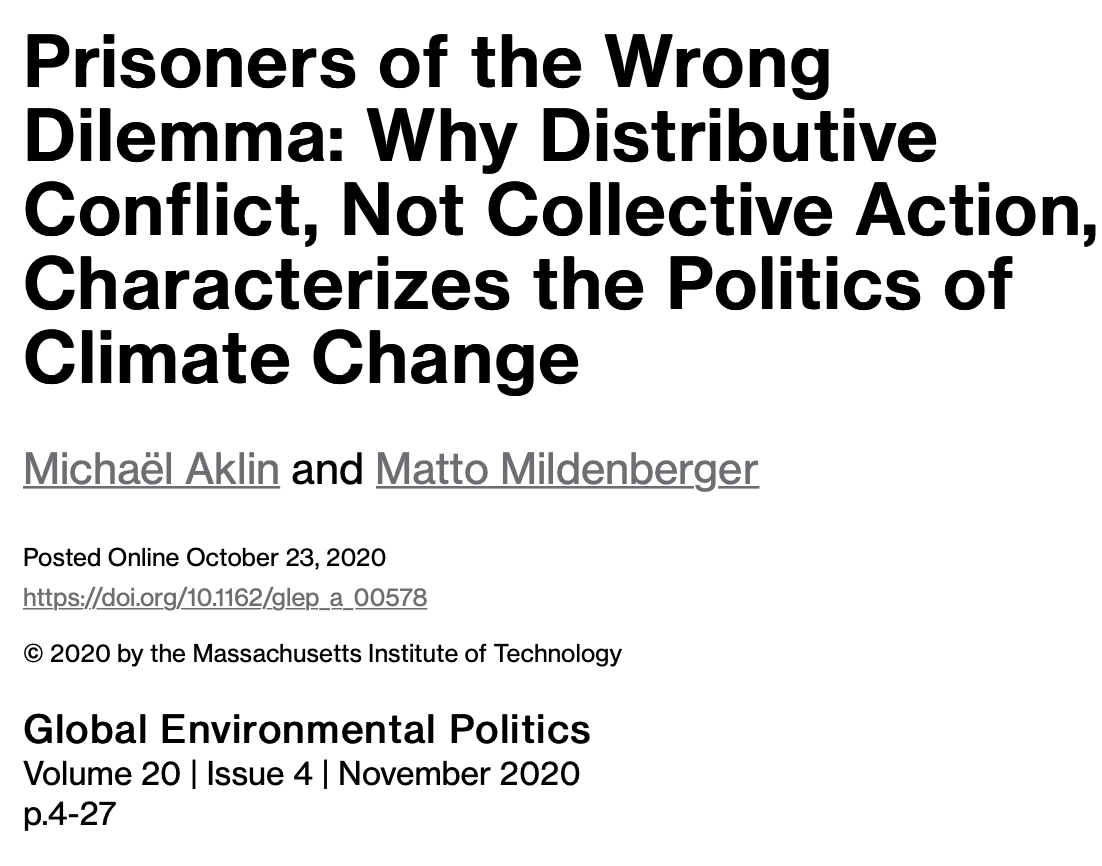
\includegraphics[width=\textwidth,height=0.7\textheight]{PD_article.png}
\caption{A recent paper arguing against the PD model}
\end{figure}
\end{frame}

\begin{frame}{Altruism}
\protect\hypertarget{altruism-1}{}
\begin{itemize}
\tightlist
\item
  The voting public, at least in rich industrial countries, does not
  favor unilateral defection from climate agreements.
\item
  This could be because of the first two factors I mentioned.
\item
  But I suspect a non-trivial factor is that people are altruistic -
  they care about others.
\item
  That is, at least given the subjectivist approach to utility we're
  using, enough to make the game not a PD.
\end{itemize}
\end{frame}

\begin{frame}{The Big Distinction}
\protect\hypertarget{the-big-distinction}{}
Is the situation you're looking at one where rational agents:

\begin{enumerate}
\tightlist
\item
  Will not cooperate without some added incentive, or
\item
  Will not be the first to cooperate without some added incentive?
\end{enumerate}

\begin{itemize}
\tightlist
\item
  If it's the first, you're in a PD; if it's the second, you may be in a
  Stag Hunt.
\item
  And then you might be better off doing some `one-time' interventions
  to get people to a new sustainable equilibrium.
\end{itemize}
\end{frame}

\begin{frame}{For Next Time}
\protect\hypertarget{for-next-time}{}
We'll move onto O'Connor's book on the origins of inequality
\end{frame}

\end{document}
